\documentclass{standalone}
\usepackage{tikz}
\begin{document}
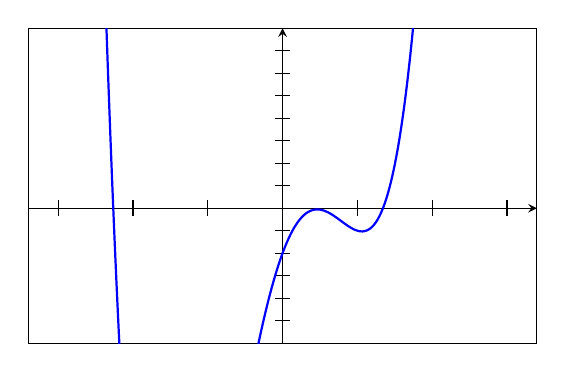
\begin{tikzpicture}[>=stealth, xscale=0.95, yscale=0.285714]
  % --- Graph of v(t) = 3t^4 - 11t^2 + 9t - 2 on -3 <= t <= 3 ---
  \def\xmin{-3.4}\def\xmax{3.4}
  \def\ymin{-6}\def\ymax{8}

  % Border around the entire image
  \draw[black] (\xmin,\ymin) rectangle (\xmax,\ymax);

  % Axes
  \draw[black, ->] (\xmin,0) -- (\xmax,0);
  \draw[black, ->] (0,\ymin) -- (0,\ymax);

  % x-axis tick marks at each integer
  \foreach \x in {-3,-2,-1,1,2,3}
    \draw[black] (\x,-0.35) -- (\x,0.35);
  % y-axis tick marks at each integer
  \foreach \y in {-6,-5,-4,-3,-2,-1,1,2,3,4,5,6,7,8}
    \draw[black] (-0.1,\y) -- (0.1,\y);

  \begin{scope}
    \clip (\xmin,\ymin) rectangle (\xmax,\ymax);

    % Exact quartic v(t) = 3t^4 - 11t^2 + 9t - 2
    \draw[blue, thick] plot[smooth, domain=-3:3, samples=200]
      ({\x}, {3*(\x)^4 - 11*(\x)^2 + 9*(\x) - 2});
  \end{scope}
\end{tikzpicture}
\end{document}
